% Options for packages loaded elsewhere
\PassOptionsToPackage{unicode}{hyperref}
\PassOptionsToPackage{hyphens}{url}
\PassOptionsToPackage{dvipsnames,svgnames,x11names}{xcolor}
\documentclass[
  11pt,
]{article}
\usepackage{xcolor}
\usepackage{amsmath,amssymb}
\setcounter{secnumdepth}{-\maxdimen} % remove section numbering
\usepackage{iftex}
\ifPDFTeX
  \usepackage[T1]{fontenc}
  \usepackage[utf8]{inputenc}
  \usepackage{textcomp} % provide euro and other symbols
\else % if luatex or xetex
  \usepackage{unicode-math} % this also loads fontspec
  \defaultfontfeatures{Scale=MatchLowercase}
  \defaultfontfeatures[\rmfamily]{Ligatures=TeX,Scale=1}
\fi
\usepackage{lmodern}
\ifPDFTeX\else
  % xetex/luatex font selection
\fi
% Use upquote if available, for straight quotes in verbatim environments
\IfFileExists{upquote.sty}{\usepackage{upquote}}{}
\IfFileExists{microtype.sty}{% use microtype if available
  \usepackage[]{microtype}
  \UseMicrotypeSet[protrusion]{basicmath} % disable protrusion for tt fonts
}{}
\makeatletter
\@ifundefined{KOMAClassName}{% if non-KOMA class
  \IfFileExists{parskip.sty}{%
    \usepackage{parskip}
  }{% else
    \setlength{\parindent}{0pt}
    \setlength{\parskip}{6pt plus 2pt minus 1pt}}
}{% if KOMA class
  \KOMAoptions{parskip=half}}
\makeatother
\usepackage{longtable,booktabs,array}
\usepackage{calc} % for calculating minipage widths
% Correct order of tables after \paragraph or \subparagraph
\usepackage{etoolbox}
\makeatletter
\patchcmd\longtable{\par}{\if@noskipsec\mbox{}\fi\par}{}{}
\makeatother
% Allow footnotes in longtable head/foot
\IfFileExists{footnotehyper.sty}{\usepackage{footnotehyper}}{\usepackage{footnote}}
\makesavenoteenv{longtable}
\usepackage{graphicx}
\makeatletter
\newsavebox\pandoc@box
\newcommand*\pandocbounded[1]{% scales image to fit in text height/width
  \sbox\pandoc@box{#1}%
  \Gscale@div\@tempa{\textheight}{\dimexpr\ht\pandoc@box+\dp\pandoc@box\relax}%
  \Gscale@div\@tempb{\linewidth}{\wd\pandoc@box}%
  \ifdim\@tempb\p@<\@tempa\p@\let\@tempa\@tempb\fi% select the smaller of both
  \ifdim\@tempa\p@<\p@\scalebox{\@tempa}{\usebox\pandoc@box}%
  \else\usebox{\pandoc@box}%
  \fi%
}
% Set default figure placement to htbp
\def\fps@figure{htbp}
\makeatother
% definitions for citeproc citations
\NewDocumentCommand\citeproctext{}{}
\NewDocumentCommand\citeproc{mm}{%
  \begingroup\def\citeproctext{#2}\cite{#1}\endgroup}
\makeatletter
 % allow citations to break across lines
 \let\@cite@ofmt\@firstofone
 % avoid brackets around text for \cite:
 \def\@biblabel#1{}
 \def\@cite#1#2{{#1\if@tempswa , #2\fi}}
\makeatother
\newlength{\cslhangindent}
\setlength{\cslhangindent}{1.5em}
\newlength{\csllabelwidth}
\setlength{\csllabelwidth}{3em}
\newenvironment{CSLReferences}[2] % #1 hanging-indent, #2 entry-spacing
 {\begin{list}{}{%
  \setlength{\itemindent}{0pt}
  \setlength{\leftmargin}{0pt}
  \setlength{\parsep}{0pt}
  % turn on hanging indent if param 1 is 1
  \ifodd #1
   \setlength{\leftmargin}{\cslhangindent}
   \setlength{\itemindent}{-1\cslhangindent}
  \fi
  % set entry spacing
  \setlength{\itemsep}{#2\baselineskip}}}
 {\end{list}}
\usepackage{calc}
\newcommand{\CSLBlock}[1]{\hfill\break\parbox[t]{\linewidth}{\strut\ignorespaces#1\strut}}
\newcommand{\CSLLeftMargin}[1]{\parbox[t]{\csllabelwidth}{\strut#1\strut}}
\newcommand{\CSLRightInline}[1]{\parbox[t]{\linewidth - \csllabelwidth}{\strut#1\strut}}
\newcommand{\CSLIndent}[1]{\hspace{\cslhangindent}#1}
\setlength{\emergencystretch}{3em} % prevent overfull lines
\providecommand{\tightlist}{%
  \setlength{\itemsep}{0pt}\setlength{\parskip}{0pt}}

\usepackage{float}\floatplacement{figure}{H}
\usepackage{etoolbox}\AtBeginEnvironment{longtable}{\scriptsize}
\setlength{\tabcolsep}{3pt}
\usepackage{setspace}\onehalfspacing
\usepackage[margin=0.9in]{geometry}
\usepackage{bookmark}
\IfFileExists{xurl.sty}{\usepackage{xurl}}{} % add URL line breaks if available
\urlstyle{same}
\hypersetup{
  pdftitle={A Foundation Model for GLP-1 Receptor Agonist-Associated NAION Risk Stratification from Reconstructed Published Evidence},
  colorlinks=true,
  linkcolor={Maroon},
  filecolor={Maroon},
  citecolor={Blue},
  urlcolor={Blue},
  pdfcreator={LaTeX via pandoc}}

\title{A Foundation Model for GLP-1 Receptor Agonist-Associated NAION
Risk Stratification from Reconstructed Published Evidence}
\usepackage{etoolbox}
\makeatletter
\providecommand{\subtitle}[1]{% add subtitle to \maketitle
  \apptocmd{\@title}{\par {\large #1 \par}}{}{}
}
\makeatother
\subtitle{Original Article}
\author{}
\date{November 23, 2026}

\begin{document}
\maketitle

\textbf{Kemar E. Green}\textsuperscript{1,2,3}\\
\textsuperscript{1}Whiting School of Engineering, Johns Hopkins
University, Baltimore, MD, USA; \textsuperscript{2}Johns Hopkins Data
Science and AI Institute, Baltimore, MD, USA;
\textsuperscript{3}NeuroAgent AI, Inc., Baltimore, MD, USA\\
Correspondence: kemarearlgreen@neuroagentai.org

\textbf{Research-prototype notice.} This work uses only published
aggregate data and computationally generated synthetic records
(synthetic\_only twins; research\_prototype=true; compliance reference
Addendum 5, DT\#9). The models are not validated for clinical,
diagnostic, treatment-selection or regulatory use, and no patient-level
health information was accessed.

\subsection{Abstract}\label{abstract}

\textbf{Background.} Observational studies and pharmacovigilance reports
link glucagon-like peptide-1 receptor agonists (GLP-1RAs), particularly
semaglutide, to nonarteritic anterior ischemic optic neuropathy (NAION),
but no tool stratifies individual risk. Whether machine learning (ML) on
published evidence, with or without synthetic digital twins, can do so
is unknown.

\textbf{Methods.} We extracted data from 73 of 169 PubMed publications
and reconstructed count-weighted patient-level data from 11
non-overlapping cohorts (3,271,499 patients; 1,425 events). Logistic
regression, random forest, XGBoost, graph neural networks and ensembles
were trained on 10\% and tested on 90\%, across 10 disjoint 10\% folds,
across training fractions of 10\% to 90\%, and by leave-one-study-out
validation. Synthetic twins were added in a factorial grid. SHAP values,
permutation tests and Benjamini-Hochberg correction were used.

\textbf{Results.} Within studies, GLP-1RA exposure was associated with
NAION (odds ratio 1.59 (95\% CI, 1.42 to 1.77)); semaglutide 1.73 (95\%
CI, 1.44 to 2.08); obesity indication 2.70 (95\% CI, 1.64 to 4.44).
XGBoost discriminated modestly (AUROC 0.656 ± 0.011; observed/expected
1.00) but fell to 0.534 in unseen studies. At the top-10\% threshold,
PPV was 0.087\% against a prevalence of 0.044\%. Neither graph or
convolutional networks, ensembles nor added vascular-score features
outperformed PubMed-only XGBoost; synthetic digital twins mainly
regularized weaker learners, and the best hybrid XGBoost gained 0.0015
AUROC. Simulated addition of optic-disc imaging raised AUROC to about
0.82 to 0.84.

\textbf{Conclusions.} Published evidence supports a reproducible
exposure signal but only modest, setting-dependent risk discrimination.
The score suits research enrichment, not treatment selection;
patient-level prospective data are required.

\subsection{Introduction}\label{introduction}

Nonarteritic anterior ischemic optic neuropathy (NAION) is the most
common acute optic nerve disease of adults older than 50
years\textsuperscript{1}, with an annual incidence of roughly 2 to 10
per 100,000 in that age group\textsuperscript{1,2}. Vision loss is
usually permanent, and the fellow eye is affected in about 15 to 21\% of
patients over several years\textsuperscript{3,4}. The leading anatomic
risk factor is a small, crowded optic disc\textsuperscript{5--7}, and
NAION is attributed to infarction of the laminar and retrolaminar optic
nerve head, with nocturnal hypotension, impaired autoregulation and a
compartment syndrome in a crowded disc among proposed
contributors\textsuperscript{8}. No treatment is
proven\textsuperscript{9,10}; decompression surgery was ineffective and
possibly harmful\textsuperscript{11}, and evidence that aspirin protects
the fellow eye is limited to conflicting observational
studies\textsuperscript{3,12,13}.

Glucagon-like peptide-1 receptor agonists (GLP-1RAs) and the dual
GIP/GLP-1 receptor agonist tirzepatide produce large reductions in
glycated hemoglobin and body weight\textsuperscript{14,15} and reduce
cardiovascular events\textsuperscript{16,17}. Since 2024, cohort studies
have reported hazard ratios of about 1.8 to 2.4 for NAION with
semaglutide\textsuperscript{18--21}, whereas other cohorts and
meta-analyses found no consistent increase\textsuperscript{22--24}.
Absolute risks are low\textsuperscript{20,25}, and proposed mechanisms
--- rapid glycemic lowering, blood-pressure and volume changes, and
intracranial-pressure effects --- remain
hypotheses\textsuperscript{26--29}. Consensus statements recommend
shared decision-making and call for identifying which patients are
susceptible\textsuperscript{25,30,31}.

No individual risk tool exists, and patient-level data remain siloed. We
assessed whether machine learning applied to reconstructed published
evidence can stratify NAION risk among GLP-1RA users, which features
matter, and whether graph neural networks, ensembles, convolutional
networks, synthetic digital twins or transfer from non-users improve on
standard models.

\subsection{Methods}\label{methods}

\subsubsection{Data sources and
extraction}\label{data-sources-and-extraction}

We searched PubMed for GLP-1RA or GIP/GLP-1RA terms combined with optic
neuropathy terms and retrieved 169 records, 60 with open-access full
text. Three extraction agents worked in parallel under a fixed schema:
patient-level rows from case reports, arm-level counts and effect
estimates from observational studies, and signal statistics and pooled
estimates from pharmacovigilance studies, pooled trials and
meta-analyses. Every value carries its PMID, an evidence level (full
text, abstract or publisher page) and a supporting quotation; unreported
values were left missing. One retracted article was
excluded\textsuperscript{32,33}.

\subsubsection{Reconstruction of patient-level
data}\label{reconstruction-of-patient-level-data}

For each of 11 cohorts with event counts in both arms we selected one
primary, non-overlapping contrast (Table 1); overlapping Danish registry
analyses and a case-control study were excluded from reconstruction.
Each arm became two rows (events, non-events) weighted by their counts,
carrying arm-level therapy and exposure and study-level indication,
region, data source, outcome definition, follow-up, mean age and
percentage female (study medians imputed with missingness indicators).
Because splitting patients uniformly at random is equivalent to binomial
or multinomial thinning of these counts, every split below operates on
individual patients without enumerating millions of rows.

\subsubsection{Models and validation}\label{models-and-validation}

We trained L2-regularized logistic regression, random forest and
XGBoost\textsuperscript{34} with count weights. Validation used (i) a
single 10\% training / 90\% test split; (ii) ten disjoint folds, each
training on a different random 10\% of patients and testing on the
remaining 90\%; (iii) training fractions from 10\% to 90\% in 10-point
steps with 10 repeats each; and (iv) leave-one-study-out validation. We
report AUROC, PR-AUC, Brier score, calibration slope and
observed-to-expected (O/E) ratio, and sensitivity, specificity,
accuracy, PPV and NPV at three thresholds fixed on training data
(Youden-optimal, top 10\%, top 20\% of predicted risk), with net
benefit\textsuperscript{35}.

\subsubsection{Graph neural networks}\label{graph-neural-networks}

Each distinct covariate pattern became a node; edges joined each node to
its k nearest neighbours in standardized feature space and linked the
exposed and comparator arms of the same study. A GraphSAGE
network\textsuperscript{36} was trained with a count-weighted binomial
loss on training counts only. We varied depth (1 to 6 layers),
neighbourhood size (5, 10, 20), edge weighting (uniform or Gaussian
kernels) and the weight of same-study links, and compared learned edge
weights through graph attention\textsuperscript{37}; configurations were
selected on folds 0 to 4 and confirmed on untouched folds 5 to 9.
Attributions used integrated gradients\textsuperscript{38}.

\subsubsection{Synthetic digital twins}\label{synthetic-digital-twins}

Twins were generated in a factorial grid\textsuperscript{39} with local
refinement\textsuperscript{40}: three generators (independent marginals;
Gaussian copula preserving feature correlations\textsuperscript{41}; a
structural model on SHAP-stable features) and their combinations, three
prior sources (fitted to the real training split, published external
priors only, or a blend), six volumes (1 to 100 times the real training
size) and synthetic shares of 10\% to 100\%, crossed with real training
fractions of 0\% to 90\%, four models and 10 repeats. Twins were never
used for testing, and generators never saw test data. Local refinement
around the best cell continued while AUROC improved by at least 0.005.

\subsubsection{Ensembles}\label{ensembles}

All combinations of two or more of logistic regression, random forest,
XGBoost and the GNN were combined by averaging, by weights from inner
cross-validation, and by stacking with a logistic meta-learner fitted on
inner out-of-fold predictions, and a cross-family ensemble averaged the
best PubMed-only, hybrid and synthetic-only models.

\subsubsection{Statistical analysis}\label{statistical-analysis}

Within-study effects were estimated with count-weighted logistic
regression with study fixed effects; marginal associations used
cluster-robust standard errors by study. SHAP values\textsuperscript{42}
were tested against null distributions from 500 refits with events
reallocated at random across arms, globally and within studies.
Published ratio estimates were pooled with DerSimonian-Laird random
effects\textsuperscript{43}. AUROC was tested against 0.5 with the
Hanley-McNeil method\textsuperscript{44}; models were compared with the
Nadeau-Bengio corrected resampled t-test\textsuperscript{45} on paired
folds and with exact McNemar tests; sensitivity, specificity, PPV, NPV
and accuracy were tested against chance with exact binomial tests. P
values within each family were adjusted with the Benjamini-Hochberg
procedure\textsuperscript{46}. Reporting follows
TRIPOD+AI\textsuperscript{47}.

\textbf{Stage 15 --- compute, energy and token use.} Energy was
estimated with the Green Algorithms method (runtime × {[}cores ×
per-core power + memory × 0.3725 W/GB{]} × PUE) for an Apple M3 Pro
laptop (PUE 1.0, package power 25 to 45 W), with run times taken from
each stage's log where available, and converted to CO2e at 0.10 to 0.70
(central 0.367) kgCO2e/kWh. Inference time was measured per 1,000
predictions. Tokens consumed by the AI assistant were recorded where
metered.

\textbf{Stage 16 --- what-if: multimodal ocular imaging.} For each
reconstructed patient, imaging features were drawn conditional on the
observed outcome (P{[}feature \textbar{} NAION{]} ∝ prior × odds ratio;
P{[}feature \textbar{} no NAION{]} = prior), independently across
features: cup-to-disc ratio categories with the published control
distribution and odds ratios (fundus photography with 25\% and OCT with
5\% adjacent-category misclassification), and hypothetical optic disc
drusen (prevalence 2\%, odds ratio 2 to 8), OCT angiography
hypoperfusion (20\%, 1.5 to 3) and serial on-treatment imaging change
(5\%, 2 to 10), with sleep apnoea (27\%, 3.28) as a non-imaging
comparator. XGBoost was trained with and without these features on five
patient-level 10\%/90\% folds for each of three generation seeds, and
the number of events needed to estimate AUROC within ±0.03 in a
prospective cohort was derived from the Hanley-McNeil variance.

\subsection{Results}\label{results}

\subsubsection{Evidence base}\label{evidence-base}

Of 169 records, 73 publications contributed data: 29 observational
studies, 17 case reports or series (18 NAION patients), 11
pharmacovigilance studies and 16 pooled-trial or meta-analytic reports
(Figure 1). Reconstruction yielded 3,271,499 patients and 1,425 events
(prevalence 0.044\%) from 11 cohorts in the United States, the Nordic
countries and the United Kingdom (Table 1). No source provided
patient-level imaging or video; case reports described fundus
photography and optical coherence tomography only as figures.

\subsubsection{Associations}\label{associations}

With study fixed effects, GLP-1RA exposure was associated with NAION
(odds ratio 1.59 (95\% CI, 1.42 to 1.77); q\textless0.001). Estimates
were 1.73 (95\% CI, 1.44 to 2.08) for semaglutide, 2.70 (95\% CI, 1.64
to 4.44) when the indication was obesity and 1.62 (95\% CI, 1.45 to
1.82) for type 2 diabetes. The association depended on the comparator:
1.81 (95\% CI, 1.54 to 2.11) against SGLT2 inhibitors and 2.35 (95\% CI,
1.74 to 3.16) against other antidiabetic drugs, but 1.03 (95\% CI, 0.57
to 1.85) against DPP-4 inhibitors and 1.14 (95\% CI, 0.94 to 1.39)
against untreated comparators. In patients with idiopathic intracranial
hypertension the direction reversed (0.43 (95\% CI, 0.22 to 0.84)). The
exposure effect was larger in studies with older participants
(interaction odds ratio 1.99 (95\% CI, 1.30 to 3.04) per 10 years;
q=0.002) and did not vary with the percentage of women (q=0.943).
Random-effects pooling of published estimates gave a ratio of 1.34 (95\%
CI, 1.16 to 1.55; I² = 87\%) (Figure 3). Patients in case reports were
younger than exposed cohort participants (median 47 vs 60 years;
q=0.016); the excess of men was not significant (q=0.274).

\subsubsection{Discrimination, calibration and
explainability}\label{discrimination-calibration-and-explainability}

Trained on 10\% of patients, XGBoost reached an AUROC of 0.657 on the
remaining 90\% with calibration slope 0.97; across ten disjoint 10\%
training folds the AUROC was 0.656 ± 0.011 and O/E 1.00 (Figure 2).
Logistic regression (0.616) and random forest (0.646) did not differ
significantly from XGBoost (all corrected q≥0.27). AUROC rose with
training fraction to a plateau near 0.67 at 40\% to 60\%. In unseen
studies, AUROC fell to 0.534. SHAP rankings were stable across folds;
permutation tests confirmed signal for exposure (q=0.004) and therapy
(q=0.015), while data source and region --- markers of setting rather
than patient risk --- carried the largest attributions.

\subsubsection{Threshold performance}\label{threshold-performance}

At the top-10\% threshold, XGBoost had sensitivity 0.35, specificity
0.82, PPV 0.087\% and NPV 99.97\% (positive likelihood ratio 2.01); at
the Youden threshold sensitivity was 0.59 and specificity 0.61.
Sensitivity and PPV exceeded chance (P\textless0.001), whereas
specificity did not exceed the value expected at the same flag rate and
accuracy remained below the no-information rate of 99.96\%. Net benefit
exceeded treat-all and treat-none strategies only at threshold
probabilities below 0.1\%. No metric differed between models (all
q≥0.99).

\subsubsection{Graph neural networks, ensembles and digital
twins}\label{graph-neural-networks-ensembles-and-digital-twins}

The GraphSAGE GNN reached an AUROC of 0.649 ± 0.014 across the 10 folds,
not different from XGBoost on identical splits (difference -0.0077;
P=0.779), with O/E 1.01. In leave-one-study-out validation its AUROC was
0.531 (P=0.034 vs 0.5). Integrated-gradient attributions ranked therapy,
data source and region highest, mirroring SHAP.

Nested tuning over 366 GNN configurations selected a SAGE network of
depth 6 with k=20 neighbours, uniform edge weighting and same-study
weight 5.0; on the untouched folds it differed from the default network
by 0.0006 AUROC (P=0.948).

Among 11 member combinations × 3 combiners, the best ensemble
(cross\_family(pubmed+hybrid+synthetic), mean) reached AUROC 0.657, a
difference of 0.0010 from the best single model (q=1.000).

In the XGBoost grid (5,310 fits), no hybrid cell improved AUROC over
PubMed-only training (0 of 162 cells with a confidence interval above
zero); the best hybrid changed AUROC by 0.0009 (95\% CI, -0.0004 to
0.0022), synthetic-only training with twins fitted to real data lost
0.010, and twins built only from published priors reached AUROC values
near 0.55. Adding twins beyond about 9 to 27 times the real training
size reduced performance.

Across the full factorial grid (45,360 configurations), 4452 hybrid or
synthetic configurations improved discrimination over PubMed-only
training after Benjamini-Hochberg correction.

Table 2 summarizes the main model families.

\subsubsection{Transport, fine-tuning and convolutional
networks}\label{transport-fine-tuning-and-convolutional-networks}

\textbf{Background-risk model transported to GLP-1RA users.} Trained on
1,983,956 non-GLP patients (740 events), background models discriminated
within non-users (AUROC 0.626 to 0.666) but much less among 1,287,543
GLP-1RA users (685 events): AUROC 0.533 to 0.597 (best, ensemble).
Observed events among GLP-1RA users exceeded background predictions (O/E
1.41 to 1.63), an independent estimate of excess risk consistent with
the within-study odds ratio. Traditional and setting features therefore
explain little of which GLP-1RA users develop NAION.

\textbf{Fine-tuning.} The best update (pooled refit; pretraining
synthetic, fine-tuning hybrid, 10\% of GLP-1RA patients) reached AUROC
0.618 in held-out GLP-1RA users with O/E 1.08. 49 configurations
improved on the pretrained background model after Benjamini-Hochberg
correction. Recalibration corrected under-prediction without changing
discrimination, as expected; synthetic fine-tuning data did not
outperform real data.

\textbf{Convolutional network.} The 1D-CNN reached AUROC 0.653 ± 0.011
across ten folds, not different from XGBoost (difference -0.0037;
P=0.782), and 0.514 in leave-one-study-out validation. Convolutions add
nothing when features lack spatial or sequential structure. Two- and
three-dimensional CNNs and multimodal fusion were not trainable: the
corpus contains one usable modality (structured tabular data derived
from text), imaging only as published figures for about six patients,
and no video.

\subsubsection{Incidence, rare-event and anomaly
models}\label{incidence-rare-event-and-anomaly-models}

\textbf{Incidence.} NAION occurred at 32.0 per 100,000 person-years
among GLP-1RA users and 17.9 among comparators (incidence rate ratio
1.79; 95\% CI, 1.61 to 1.99; Mantel-Haenszel ratio stratified by study
1.73), a rate difference of 14.1 per 100,000 person-years. Both rates
lie within or above the published background range for adults aged 50
years or older\textsuperscript{1,2}. The ratio was 1.84 in type 2
diabetes and 0.43 in idiopathic intracranial hypertension, and Poisson
models with study fixed effects showed heterogeneity of the exposure
effect by study age band (P=\textless0.001), indication
(P=\textless0.001), drug (P=0.002), comparator (P=0.026) and follow-up
(P=\textless0.001) but not by the percentage of women (P=0.756). Because
age is a study-level attribute and person-years were reported by only
two studies, these strata describe settings rather than individual
patients.

\textbf{Rare-event and anomaly-detection models.} A Poisson rate model
with a person-time offset (AUROC 0.652), King-Zeng corrected logistic
regression (0.655) and incidence-anchored XGBoost (0.657) matched
standard XGBoost (0.656); class weighting required prior correction to
restore calibration, and a focal-loss network was miscalibrated. Anomaly
detectors trained only on patients without NAION performed near chance
(AUROC 0.413 to 0.575), because patients with and without NAION from the
same study arm share identical features in reconstructed aggregate data;
anomaly methods need individual-level covariates.

\subsubsection{Detection within GLP-1RA users and
non-users}\label{detection-within-glp-1ra-users-and-non-users}

\textbf{Performance within GLP-1RA users and within non-users.} Trained
on mixed data, every model discriminated better among non-users (AUROC
0.577 to 0.674) than among GLP-1RA users (0.511 to 0.600; best, xgb).
The within-group difference in AUROC was significant after correction
for 0 of 9 models. Together with the under-prediction of a background
model in GLP-1RA users, this indicates that the features available in
published data capture background NAION risk but little of what
determines which GLP-1RA users develop NAION.

\subsubsection{Vascular score features and a proposed NAION-adapted
score}\label{vascular-score-features-and-a-proposed-naion-adapted-score}

\textbf{Validated vascular score as a feature.} Only three ABCD2/ABCD3-I
items could be derived: age 60 years or older (7 of 11 studies, from
study mean age), blood pressure (5 of 11, using hypertension prevalence
as a proxy) and diabetes (11 of 11); clinical features, symptom
duration, dual events and imaging are specific to transient ischemic
attack. Adding the partial items to XGBoost changed AUROC by -0.0019
(P=0.917). The partial score alone, in studies with all items, reached
AUROC 0.545.

\textbf{Proposed NAION-adapted points score.} Fitting point weights to
the reconstructed data produced implausible protective signs for
hypertension, diabetes and GLP-1RA exposure, because these items vary
only between studies; we therefore report this fit only as a
demonstration of ecological bias. A literature-informed version assigned
points from published patient-level ratios (male sex, hypertension,
hyperlipidemia, diabetes, coronary heart disease and sleep
apnea\textsuperscript{48}) and from our within-study GLP-1RA estimates
(indication-specific), with age carried from the ABCD2 convention: male
sex 2 points, hypertension 1 point, hyperlipidemia 1 point, diabetes 2
points, coronary heart disease 2 points, sleep apnea 5 points, age ge60
1 point, cdr le 0.20 post exposure fellow eye 16 points, cdr 0.21 0.40
post exposure fellow eye 8 points, glp1ra t2d 2 points, glp1ra obesity 4
points. On setting-level data it ranked cohorts poorly (AUROC 0.417;
difference from XGBoost -0.240), as expected when settings with more
vascular risk factors recorded fewer events; the score requires
prospective, patient-level calibration, including disc morphology.

\textbf{Limitations of the partial score.} only A, B and D of
ABCD2/ABCD3-I are derivable; C, duration, dual-TIA and imaging items are
TIA-specific; A and B are study-level proxies (age from study mean with
assumed SD 12; hypertension diagnosis for BP \textgreater= 140/90); A
available for 7/11 and B for 5/11 studies; remaining values imputed and
flagged; both arms of a study share the same A and B, so the score
cannot separate exposed from unexposed patients within a study; any
apparent importance reflects between-setting differences, not individual
patient risk.

\textbf{Cup-to-disc ratio.} No source reported a pre-treatment
(pre-GLP-1RA) cup-to-disc ratio. In the case reports, disc status was
recorded at or after NAION diagnosis, usually in the unaffected fellow
eye. The largest source, a 16-center case-control study of 1,812
unaffected fellow eyes, found a fellow-eye ratio of 0.20 or less in 54\%
of patients with NAION versus 9\% of controls (odds ratio 46.3; 95\% CI,
22.9 to 93.4; ratio 0.21 to 0.40: 6.8; 3.5 to 13.2) and no difference
between semaglutide users, other GLP-1RA users and unexposed
patients\textsuperscript{49}. We therefore entered the cup-to-disc ratio
as the highest-weighted item of the proposed score but labelled it a
post-exposure fellow-eye measurement: disc anatomy is structurally
stable and the fellow eye is the accepted proxy, yet this is weaker
evidence than a baseline measured before GLP-1RA initiation, and it
could not be validated in the cohort data. The same limitation applies
to NAION without GLP-1RA exposure: the classic and recent disc-at-risk
studies measured the cup-to-disc ratio after the event, in fellow eyes
or in affected eyes after edema resolved\textsuperscript{5--7,49}, and
none had a measurement taken before NAION. Because both groups share
this post-event design, the comparison between exposed and unexposed
NAION is balanced, but no source supports a truly prospective
(pre-event) estimate of disc-related risk. Baseline optic disc
photography or OCT before GLP-1RA initiation in a prospective cohort
would close this gap.

\textbf{With versus without ABCD features across all experiments.} Over
455 paired comparisons using identical splits and seeds, adding the
partial ABCD items changed AUROC by 0.0016 on average; 0 comparisons
differed after Benjamini-Hochberg correction.

\subsubsection{Feature combinations and the compounding
hypothesis}\label{feature-combinations-and-the-compounding-hypothesis}

\textbf{Feature combinations and the compounding hypothesis.} Across all
511 combinations of nine feature groups, the largest Shapley
contributions to XGBoost AUROC came from setting (0.0350), duration
(0.0290), sex (0.0270), drug (0.0212). For the hypothesis that
individually negligible features contribute in combination, no feature
group met the prespecified criteria; no pair showed significant positive
interaction. For an optional-input calculator, a single XGBoost trained
with random feature-group dropout differed from a bank of dedicated
sub-models by -0.0121 AUROC on average across input patterns.

\subsubsection{Compute footprint and imaging
what-if}\label{compute-footprint-and-imaging-what-if}

\textbf{Compute, energy and token use.} All model training and inference
ran locally on one laptop (Apple M3 Pro, 11 cores, 18 GB). Across every
experiment the analyses used 7.6 wall-clock hours and 62.6 core-hours
(87\% of run time measured from logs, the rest estimated), consuming an
estimated 0.25 kWh (range 0.19 to 0.31) and emitting 92 g CO2e at the US
average grid intensity (range 19 to 215 g), about 0.5 km of car travel.
The largest single consumer was the full-factorial twins (2.4 h).
Inference was negligible: logreg 0.75 ms, rf 26.68 ms, xgb 1.69 ms per
1,000 patients. The AI assistant used for retrieval, extraction and
drafting consumed at least 764,562 tokens in the four metered extraction
and literature agents; tokens of the main session were not metered, and
assistant inference energy, which occurs in remote data centres, is not
included in these totals.

\textbf{What-if: adding ocular imaging (simulation).} Imaging values
were simulated for the reconstructed patients conditional on their
observed outcome. Adding cup-to-disc ratio from fundus photographs, with
published odds ratios\textsuperscript{49} and 25\% photographic
misclassification, raised AUROC from 0.653 to 0.770; OCT-measured ratio
reached 0.818. Adding hypothetical effects for optic disc drusen, OCT
angiography perfusion and serial on-treatment imaging reached 0.840
(range across hypothetical effect sizes 0.825 to 0.876), and 0.854 with
sleep apnoea added; sleep apnoea alone reached 0.708. Positive
predictive value at the top-10\% threshold rose from 0.098\% to 0.262\%,
still below 1\% because NAION is rare. A prospective cohort would need
about 263 NAION events, roughly 604,000 GLP-1RA initiators at the
observed incidence, to estimate AUROC within ±0.03; a case-control
design enriched for NAION would need far fewer imaged patients. These
figures are simulations that assume conditional independence of features
and, for drusen, OCT angiography and serial imaging, effect sizes that
have not been measured.

\subsection{Discussion}\label{discussion}

Published evidence on GLP-1RAs and NAION contains a consistent exposure
signal: within the same studies, exposed patients had roughly 1.6 times
the odds of NAION, and the estimate was higher for semaglutide and for
obesity indications. Machine learning on the same evidence, however,
discriminated only modestly, and most of what it learned was where a
patient was treated rather than who the patient was. Discrimination
collapsed toward chance in studies the model had not seen, and the
strongest attributions went to data source and region. More flexible
learners --- graph neural networks, ensembles and synthetic digital
twins --- did not change this picture.

The threshold metrics show what this means in practice. Sensitivity and
PPV beat chance, so the score enriches for cases roughly twofold, which
is an advantage for selecting patients for closer surveillance or for
enrolment in research. Absolute PPV, however, stayed below 0.1\%: about
one in 1,100 flagged patients would develop NAION. Specificity added
nothing beyond the flag rate, accuracy was uninformative because the
outcome is rare, and the high NPV mainly reflected the low prevalence.
Net benefit was positive only at threshold probabilities suited to
low-risk actions such as a dilated examination or optical coherence
tomography before treatment, counselling, or slower dose escalation,
consistent with recent consensus recommendations\textsuperscript{25,30}.

The intended clinical question is whether a validated score can identify
patients who should start antiplatelet therapy. These data cannot answer
it. Risk prediction is not treatment-effect prediction; none of the
extracted cohorts or case reports recorded antiplatelet exposure, NAION
is not primarily thromboembolic, and the evidence for aspirin after
NAION is limited. At the observed PPV, treating every flagged patient
would expose roughly a thousand people to bleeding risk per event that
occurs, before any benefit is assumed. Answering the question requires
prospective validation with patient-level predictors (disc morphology,
sleep apnoea, nocturnal hypotension, dose escalation) followed by a
risk-stratified trial with bleeding as a co-primary safety outcome.

Synthetic twins helped only weak learners. In the full factorial
experiment, thousands of hybrid configurations improved logistic
regression, consistent with regularization, but the best hybrid XGBoost
gained only 0.0015 AUROC; twins built from published priors alone
produced little more than chance discrimination, and fine-tuning a
background model worked only with real GLP-1RA data. Twins cannot create
patient-level information that the source data do not contain.

The limiting factor is the feature set, not the learner. In simulation,
adding cup-to-disc ratio from fundus photographs or OCT, with published
effect sizes, raised AUROC from about 0.65 to 0.77 to 0.82, and
plausible additional imaging reached about 0.84; even then positive
predictive value stayed below 1\%. A prospective cohort of GLP-1RA
initiators with baseline optic-disc imaging, which no published study
has reported, is therefore the most informative next step. The entire
analysis used about 0.25 kWh of local compute, so the environmental cost
of the modelling itself is negligible relative to the data collection it
motivates.

We describe this work as a foundation machine learning model in the
sense of a base layer: it fixes the outcome definition, the
reconstructed evidence base, the validation protocol and a benchmark
(AUROC about 0.66 within settings, about 0.53 across settings) against
which every later module must be judged. It is not a large pretrained
model. The intended next layers are encoders for optic-disc photography
and OCT and separately pretrained components such as an oculomotor world
model, a learned generative model of eye-movement dynamics adapted from
Ha and Schmidhuber\textsuperscript{50}, trained on synthetic
eye-movement data and sharing no variables with the present data,
combined in a multimodal neuro-ophthalmic foundation model. No transfer
between components was performed or evaluated here; it requires patients
with linked risk factors, imaging and oculomotor recordings.

This study has limitations. Predictors were arm- or study-level, so
associations with age, sex and setting are ecological. Reconstructed
patients share covariate patterns, which makes thresholds coarse.
Outcome definitions differed (one cohort reported ischemic optic
neuropathy), TriNetX cells below 10 were masked, several studies were
available only as abstracts, and overlapping registries were handled by
selection rather than by individual linkage. No imaging was available,
so multimodal and computer-vision models could not be trained. All
results are retrospective and in silico.

In conclusion, ML on published evidence confirms a modest, reproducible
association between GLP-1RA exposure and NAION and yields a
research-grade enrichment score, not a treatment-selection tool.
Patient-level prospective data are the necessary next step.

\textbf{Use of AI tools.} Literature retrieval, data extraction,
analysis code, figures and the first draft of this manuscript were
produced with an AI assistant (Claude, Anthropic) working under the
direction of the authors. Every extracted value carries a source PMID
and evidence quote. The authors are responsible for verifying all
content before submission. AI tools are not authors.

\subsection{Tables and figures}\label{tables-and-figures}

\begin{longtable}[]{@{}
  >{\raggedright\arraybackslash}p{(\linewidth - 14\tabcolsep) * \real{0.1758}}
  >{\raggedright\arraybackslash}p{(\linewidth - 14\tabcolsep) * \real{0.1152}}
  >{\raggedright\arraybackslash}p{(\linewidth - 14\tabcolsep) * \real{0.0606}}
  >{\raggedright\arraybackslash}p{(\linewidth - 14\tabcolsep) * \real{0.0848}}
  >{\raggedright\arraybackslash}p{(\linewidth - 14\tabcolsep) * \real{0.1697}}
  >{\raggedright\arraybackslash}p{(\linewidth - 14\tabcolsep) * \real{0.1212}}
  >{\raggedright\arraybackslash}p{(\linewidth - 14\tabcolsep) * \real{0.1273}}
  >{\raggedright\arraybackslash}p{(\linewidth - 14\tabcolsep) * \real{0.1455}}@{}}
\caption{Cohorts reconstructed into count-weighted patient-level data
(one primary, non-overlapping contrast per study).}\tabularnewline
\toprule\noalign{}
\begin{minipage}[b]{\linewidth}\raggedright
Study
\end{minipage} & \begin{minipage}[b]{\linewidth}\raggedright
Setting
\end{minipage} & \begin{minipage}[b]{\linewidth}\raggedright
Region
\end{minipage} & \begin{minipage}[b]{\linewidth}\raggedright
Population
\end{minipage} & \begin{minipage}[b]{\linewidth}\raggedright
Exposure
\end{minipage} & \begin{minipage}[b]{\linewidth}\raggedright
Comparator
\end{minipage} & \begin{minipage}[b]{\linewidth}\raggedright
Exposed, events/N
\end{minipage} & \begin{minipage}[b]{\linewidth}\raggedright
Comparator, events/N
\end{minipage} \\
\midrule\noalign{}
\endfirsthead
\toprule\noalign{}
\begin{minipage}[b]{\linewidth}\raggedright
Study
\end{minipage} & \begin{minipage}[b]{\linewidth}\raggedright
Setting
\end{minipage} & \begin{minipage}[b]{\linewidth}\raggedright
Region
\end{minipage} & \begin{minipage}[b]{\linewidth}\raggedright
Population
\end{minipage} & \begin{minipage}[b]{\linewidth}\raggedright
Exposure
\end{minipage} & \begin{minipage}[b]{\linewidth}\raggedright
Comparator
\end{minipage} & \begin{minipage}[b]{\linewidth}\raggedright
Exposed, events/N
\end{minipage} & \begin{minipage}[b]{\linewidth}\raggedright
Comparator, events/N
\end{minipage} \\
\midrule\noalign{}
\endhead
\bottomrule\noalign{}
\endlastfoot
Hathaway 2024\textsuperscript{18} & Single center & US & T2D &
Semaglutide & Other antidiabetic & 46/555 & 23/1,134 \\
Grauslund 2024\textsuperscript{19} & National registry & Nordic & T2D &
Semaglutide & No GLP-1RA & 67/106,454 & 151/317,698 \\
Simonsen 2025\textsuperscript{51} & National registry & Nordic & T2D &
Semaglutide & SGLT2i & 8/16,860 & 7/34,153 \\
Hsu 2025\textsuperscript{21} & EHR network & US & T2D & Semaglutide &
Other antidiabetic & 45/174,584 & 29/174,584 \\
Wang 2025\textsuperscript{52} & EHR network & US & T2D & Semaglutide or
tirzepatide & Other antidiabetic & 35/79,699 & 19/79,699 \\
Ramsey 2025\textsuperscript{53} & EHR network & US & T2D & GLP-1RA class
& No GLP-1RA & 96/185,066 & 79/185,066 \\
Tesfaye 2026\textsuperscript{54} & Claims & US & T2D & GLP-1RA class &
SGLT2i & 270/482,912 & 144/482,912 \\
Heberer 2026\textsuperscript{20} & VA EHR & US & T2D & Semaglutide &
SGLT2i & 30/11,478 & 143/90,883 \\
Noh 2026\textsuperscript{55} & Primary-care EHR & UK & T2D & GLP-1RA
class & DPP-4i & 14/106,858 & 53/416,369 \\
Al-Harbi 2026\textsuperscript{56} & EHR network & US & IIH & GLP-1RA
class & No GLP-1RA & 12/15,559 & 28/15,560 \\
Ueda 2026\textsuperscript{57} & National registry & Nordic & T2D &
GLP-1RA class & SGLT2i & 62/107,518 & 64/185,898 \\
\end{longtable}

\begin{longtable}[]{@{}
  >{\raggedright\arraybackslash}p{(\linewidth - 14\tabcolsep) * \real{0.3333}}
  >{\raggedright\arraybackslash}p{(\linewidth - 14\tabcolsep) * \real{0.1179}}
  >{\raggedright\arraybackslash}p{(\linewidth - 14\tabcolsep) * \real{0.0769}}
  >{\raggedright\arraybackslash}p{(\linewidth - 14\tabcolsep) * \real{0.1590}}
  >{\raggedright\arraybackslash}p{(\linewidth - 14\tabcolsep) * \real{0.0718}}
  >{\raggedright\arraybackslash}p{(\linewidth - 14\tabcolsep) * \real{0.0359}}
  >{\raggedright\arraybackslash}p{(\linewidth - 14\tabcolsep) * \real{0.1077}}
  >{\raggedright\arraybackslash}p{(\linewidth - 14\tabcolsep) * \real{0.0974}}@{}}
\caption{Model performance by family. AUROC values for 10×10\% folds are
mean ± SD; thresholds fixed on training data; PPV and NPV as
percentages. LOSO, leave-one-study-out; O/E, observed-to-expected
events.}\tabularnewline
\toprule\noalign{}
\begin{minipage}[b]{\linewidth}\raggedright
Model
\end{minipage} & \begin{minipage}[b]{\linewidth}\raggedright
Training data
\end{minipage} & \begin{minipage}[b]{\linewidth}\raggedright
AUROC 10/90
\end{minipage} & \begin{minipage}[b]{\linewidth}\raggedright
AUROC 10×10\% folds
\end{minipage} & \begin{minipage}[b]{\linewidth}\raggedright
AUROC LOSO
\end{minipage} & \begin{minipage}[b]{\linewidth}\raggedright
O/E
\end{minipage} & \begin{minipage}[b]{\linewidth}\raggedright
Sens/Spec top 10\%
\end{minipage} & \begin{minipage}[b]{\linewidth}\raggedright
PPV/NPV top 10\%
\end{minipage} \\
\midrule\noalign{}
\endfirsthead
\toprule\noalign{}
\begin{minipage}[b]{\linewidth}\raggedright
Model
\end{minipage} & \begin{minipage}[b]{\linewidth}\raggedright
Training data
\end{minipage} & \begin{minipage}[b]{\linewidth}\raggedright
AUROC 10/90
\end{minipage} & \begin{minipage}[b]{\linewidth}\raggedright
AUROC 10×10\% folds
\end{minipage} & \begin{minipage}[b]{\linewidth}\raggedright
AUROC LOSO
\end{minipage} & \begin{minipage}[b]{\linewidth}\raggedright
O/E
\end{minipage} & \begin{minipage}[b]{\linewidth}\raggedright
Sens/Spec top 10\%
\end{minipage} & \begin{minipage}[b]{\linewidth}\raggedright
PPV/NPV top 10\%
\end{minipage} \\
\midrule\noalign{}
\endhead
\bottomrule\noalign{}
\endlastfoot
Logistic regression (L2) & PubMed only & 0.627 & 0.616 ± 0.010 & 0.528 &
1.01 & 0.26/0.85 & 0.075\%/99.96\% \\
Random forest & PubMed only & 0.642 & 0.646 ± 0.014 & 0.531 & 1.00 &
0.31/0.85 & 0.096\%/99.96\% \\
XGBoost & PubMed only & 0.657 & 0.656 ± 0.011 & 0.534 & 1.00 & 0.35/0.82
& 0.087\%/99.97\% \\
Mean ensemble (LR+RF+XGB) & PubMed only & 0.657 & 0.656 ± 0.011 & --- &
--- & 0.31/0.86 & 0.101\%/99.97\% \\
GNN (GraphSAGE, 2 layers) & PubMed only & 0.647 & 0.649 ± 0.014 & 0.531
& 1.01 & 0.35/0.82 & 0.086\%/99.97\% \\
GNN tuned (SAGE, depth 6, k=20, uniform, study weight 5.0) & PubMed only
& --- & 0.657 (untouched folds) & 0.541 & 1.03 & --- & --- \\
xgb --- pubmed only & PubMed only & --- & 0.667 (all fractions) & --- &
1.00 & --- & --- \\
xgb --- hybrid (copula + structural generators, published priors, 100×,
10\% synthetic) & Hybrid & --- & 0.669 (all fractions) & --- & 1.01 &
--- & --- \\
ensemble --- synthetic only (copula generator, real-data priors, 9×,
100\% synthetic) & Synthetic only & --- & 0.664 (all fractions) & --- &
1.01 & --- & --- \\
ensemble --- synthetic only, 0\% real (copula generator, 100×) &
Published priors only & --- & 0.569 (all real data as test) & --- & 1.11
& --- & --- \\
Ensemble cross\_family(pubmed+hybrid+synthetic) (mean) & PubMed only &
--- & 0.657 ± 0.010 & --- & 1.01 & --- & --- \\
Ensemble logreg+xgb (mean) & PubMed only & --- & 0.657 ± 0.008 & --- &
1.00 & --- & --- \\
\end{longtable}

\begin{figure}
\centering
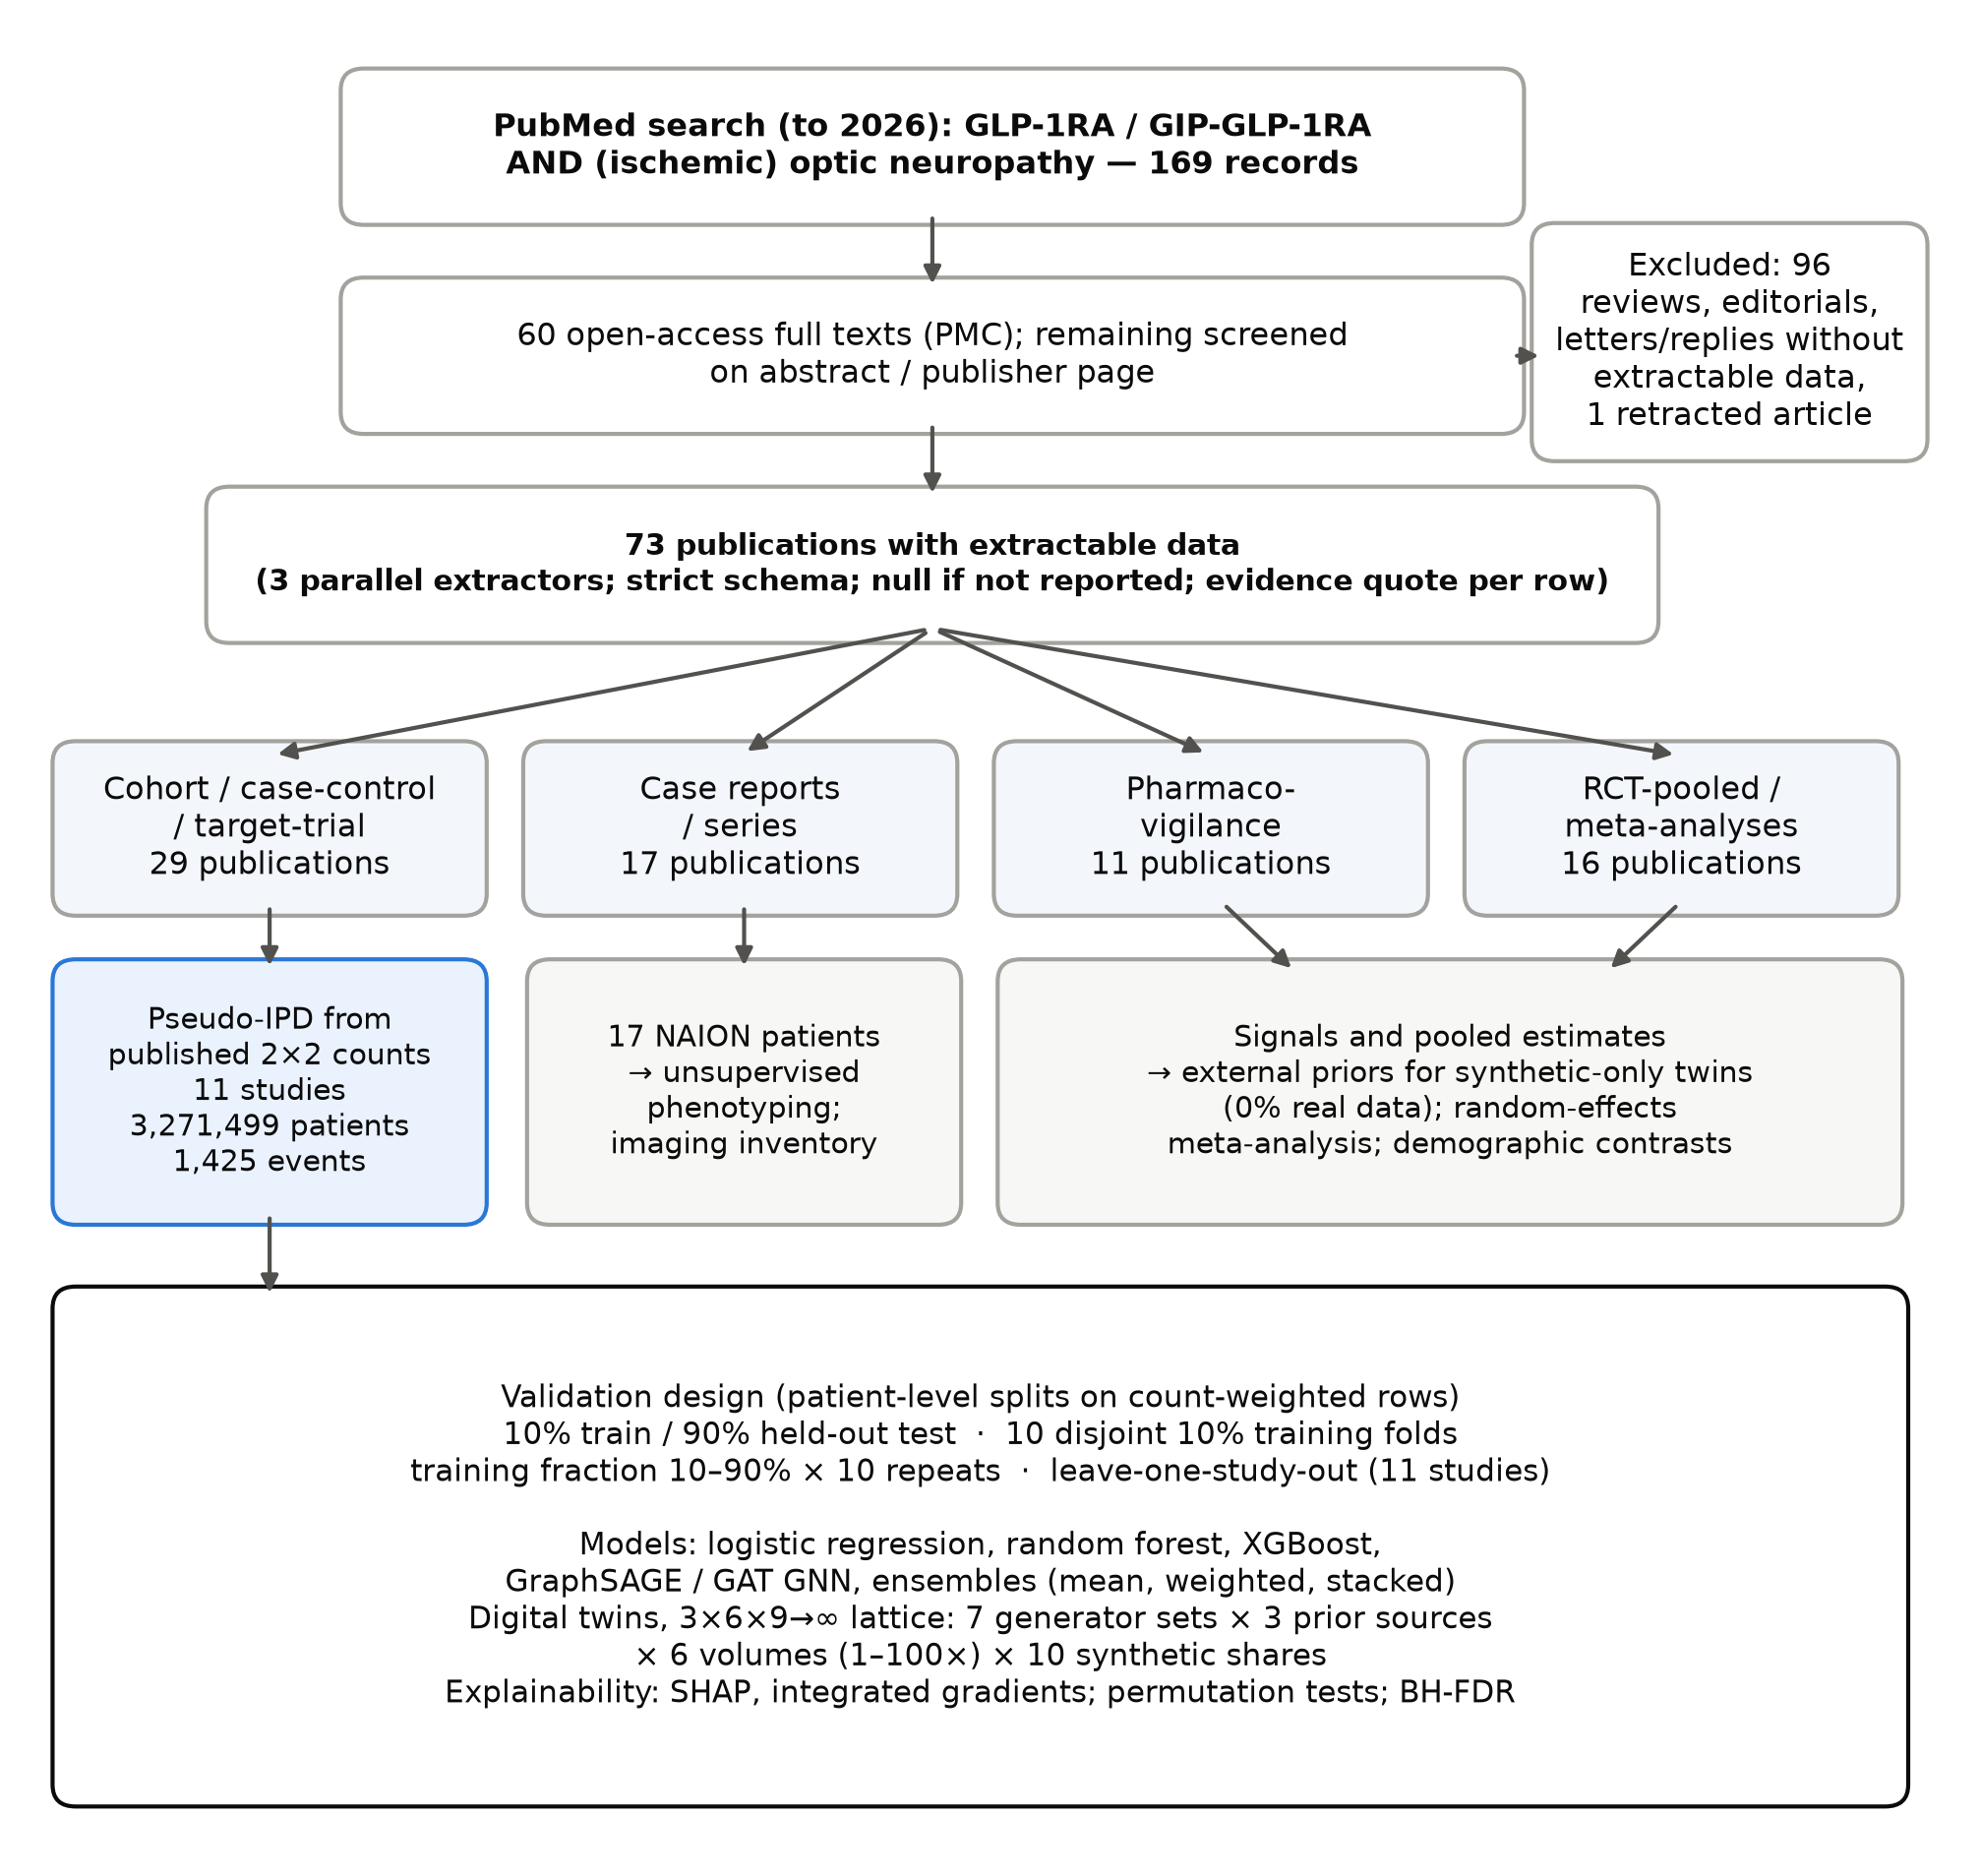
\includegraphics[width=1\linewidth,height=\textheight,keepaspectratio,alt={Study flow and validation design.}]{figures/fig1_study_flow.png}
\caption{Study flow and validation design.}
\end{figure}

\begin{figure}
\centering
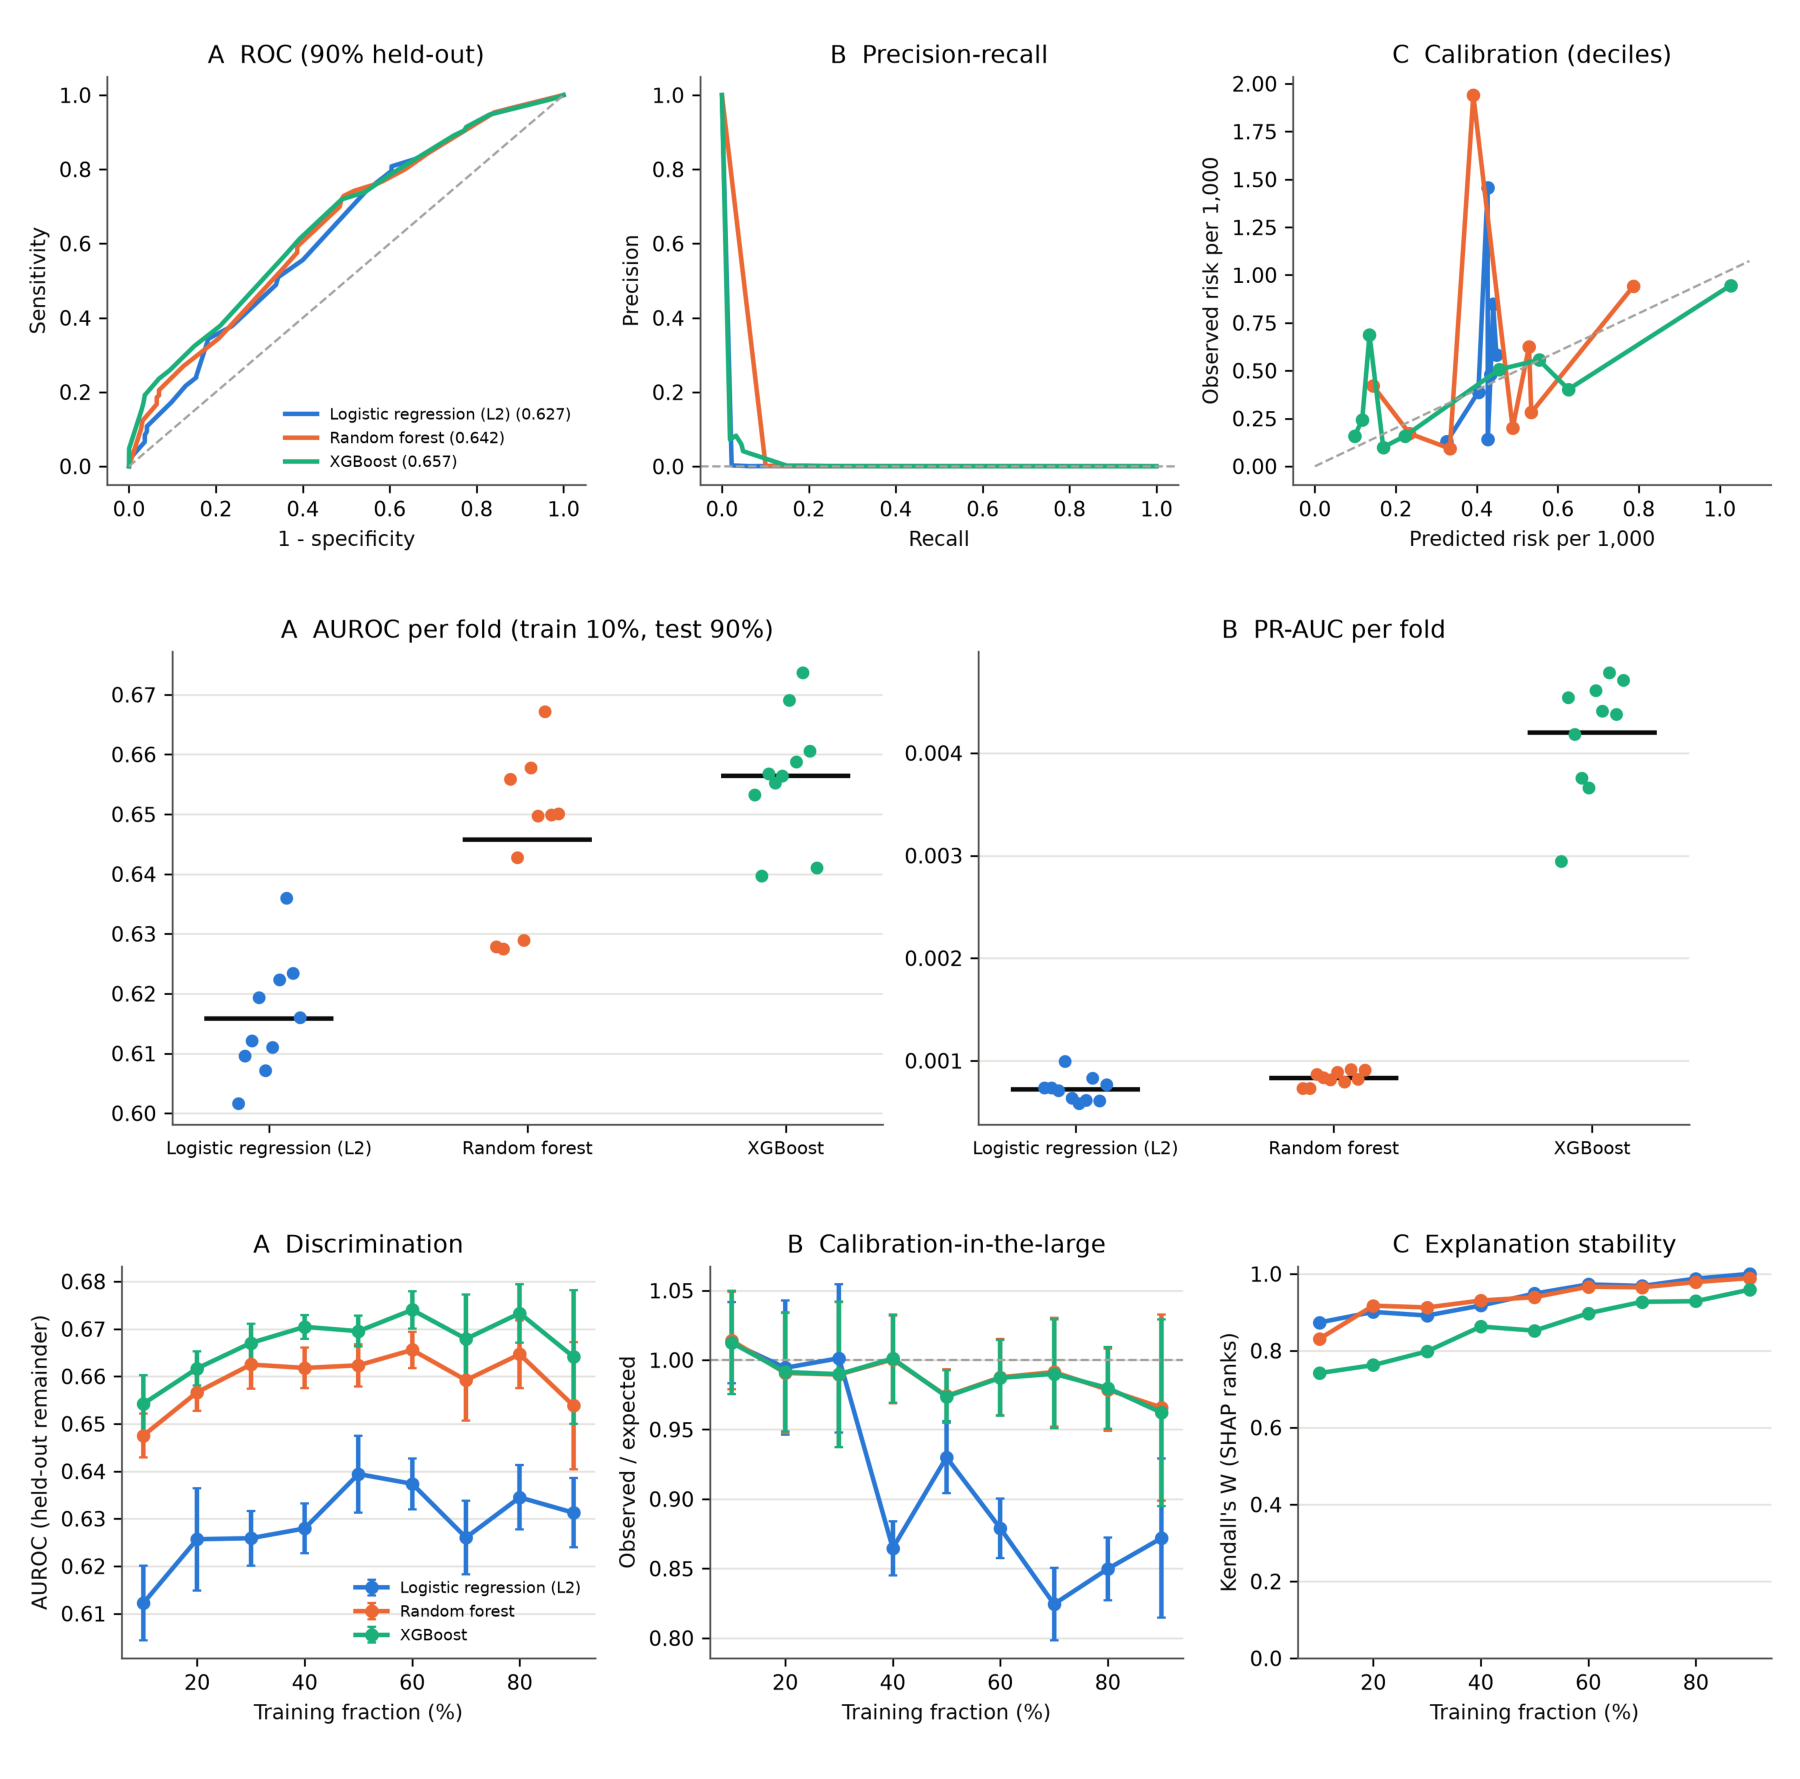
\includegraphics[width=1\linewidth,height=\textheight,keepaspectratio,alt={Discrimination and calibration of PubMed-only models: (top) receiver-operating-characteristic, precision-recall and decile calibration on the 90\% hold-out after training on 10\%; (middle) AUROC and PR-AUC across ten disjoint 10\% training folds; (bottom) AUROC, calibration-in-the-large and SHAP-rank stability across training fractions of 10\% to 90\%.}]{figures/fig2_performance.png}
\caption{Discrimination and calibration of PubMed-only models: (top)
receiver-operating-characteristic, precision-recall and decile
calibration on the 90\% hold-out after training on 10\%; (middle) AUROC
and PR-AUC across ten disjoint 10\% training folds; (bottom) AUROC,
calibration-in-the-large and SHAP-rank stability across training
fractions of 10\% to 90\%.}
\end{figure}

\begin{figure}
\centering
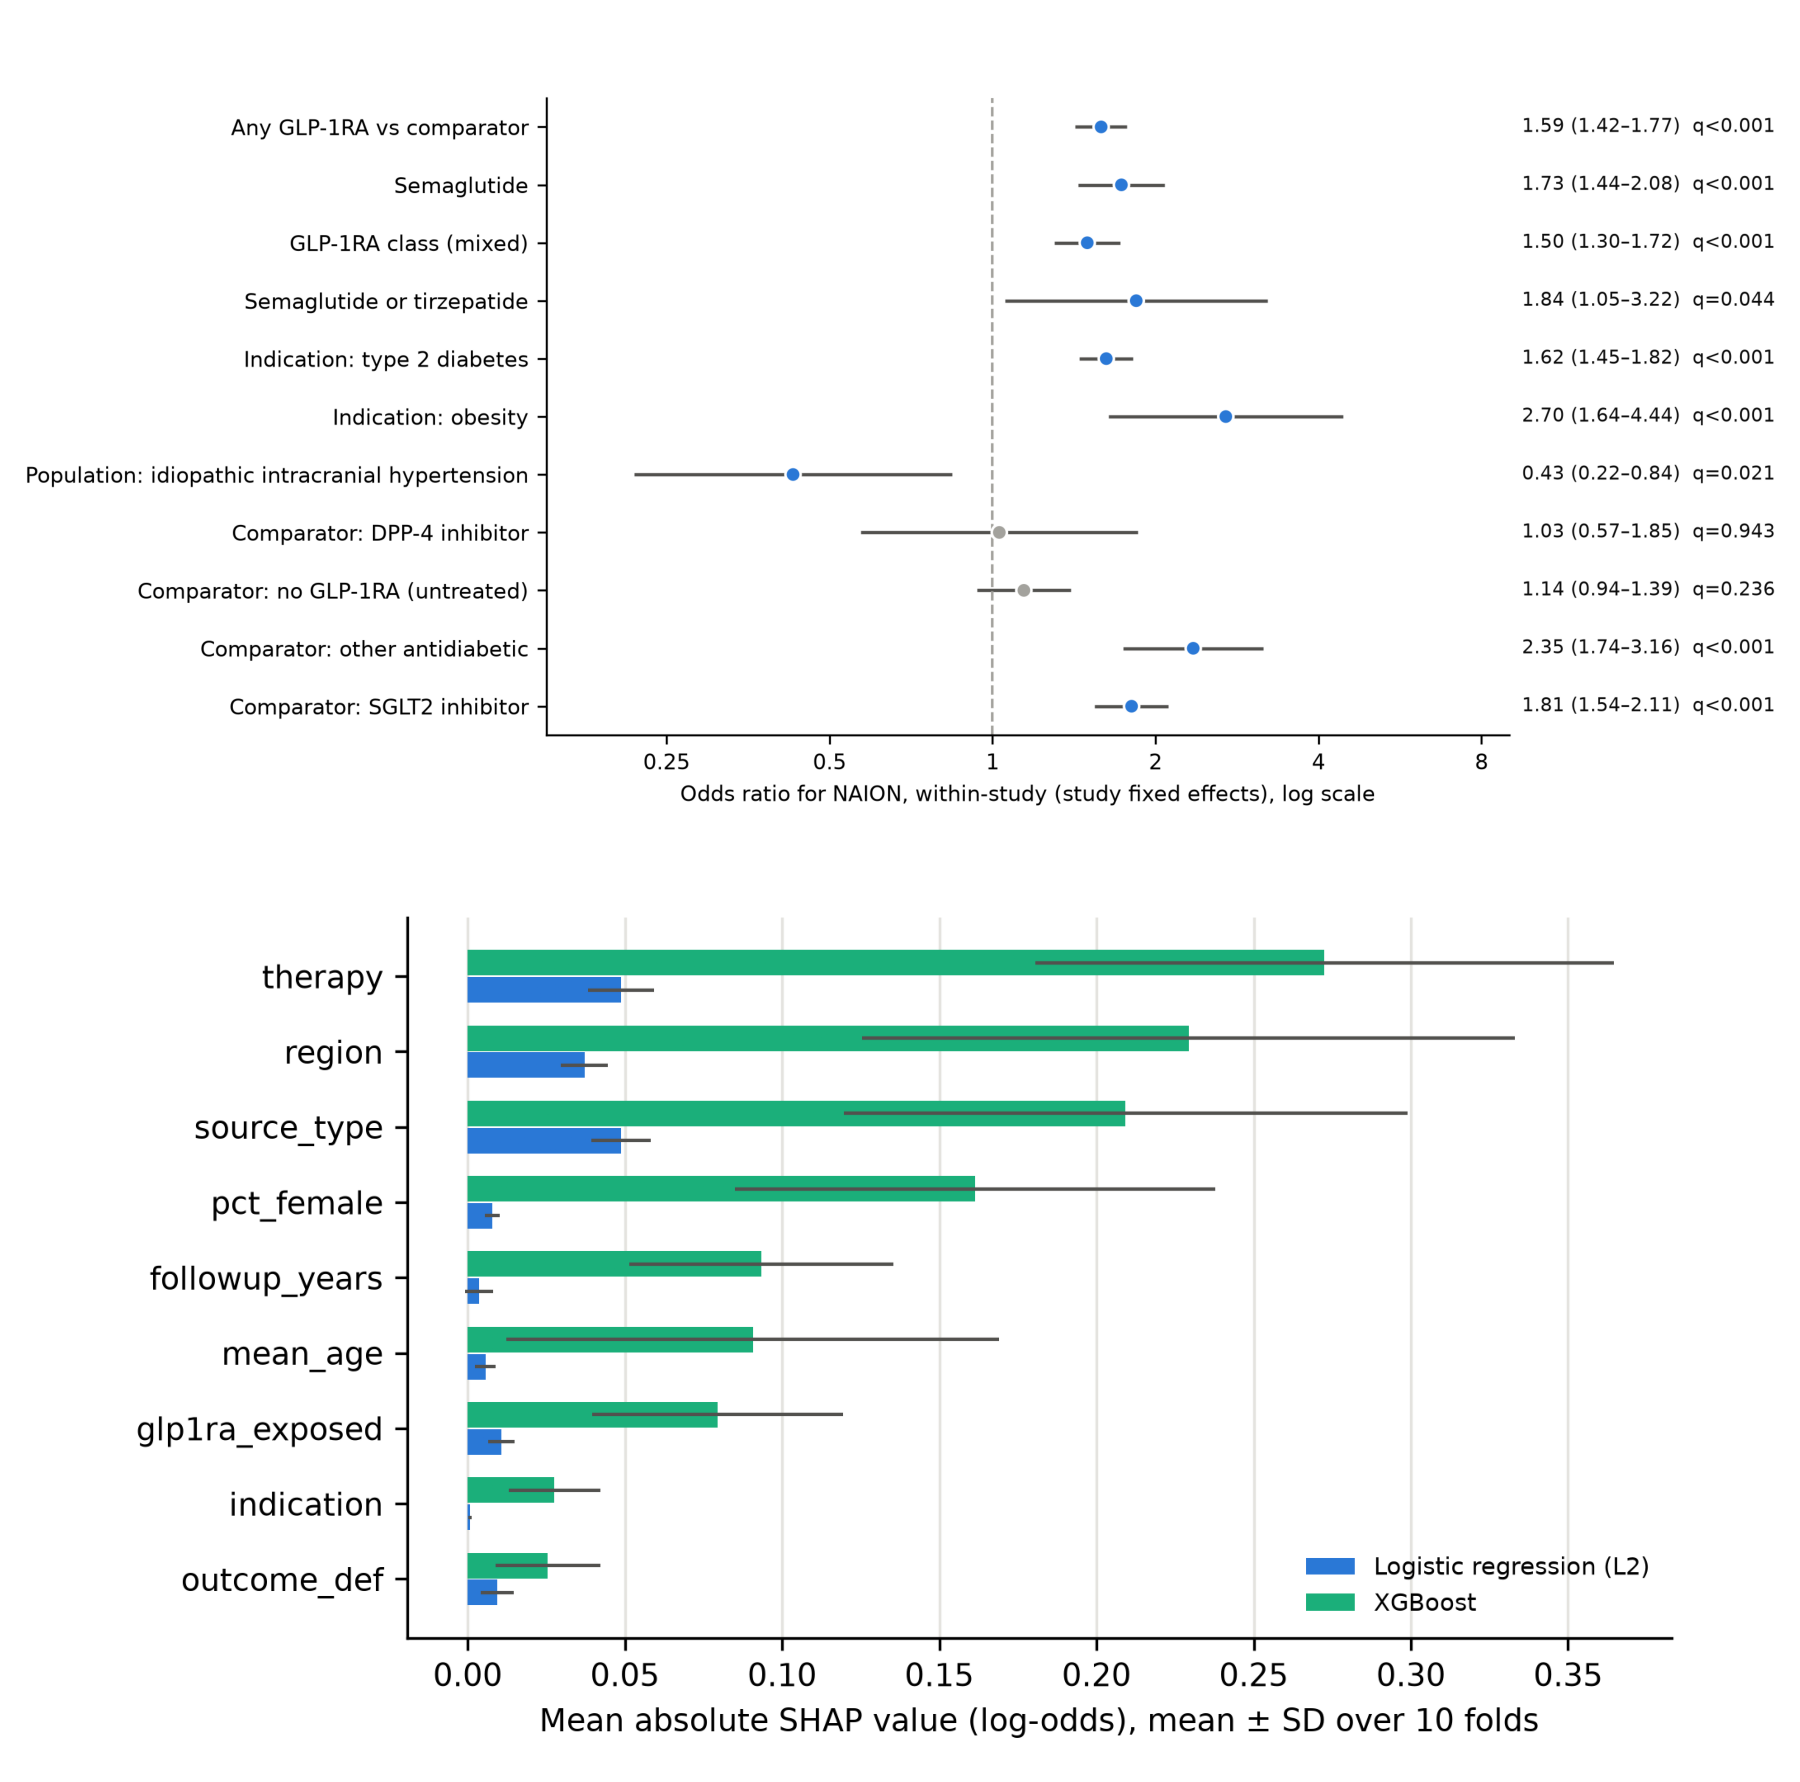
\includegraphics[width=1\linewidth,height=\textheight,keepaspectratio,alt={(Top) Within-study odds ratios for NAION with study fixed effects (blue, q\textless0.05 after Benjamini-Hochberg correction). (Bottom) SHAP importance (mean ± SD over ten folds) for three model types.}]{figures/fig3_effects_explainability.png}
\caption{(Top) Within-study odds ratios for NAION with study fixed
effects (blue, q\textless0.05 after Benjamini-Hochberg correction).
(Bottom) SHAP importance (mean ± SD over ten folds) for three model
types.}
\end{figure}

The Supplementary Appendix (the full preprint) contains all additional
tables and figures: data inventory and modalities; case-level
phenotyping and meta-regression; every P value (within-study and
marginal associations, SHAP permutation tests, meta-analysis,
demographics, ML experiments); threshold metrics for all models;
training-fraction sweeps; GNN depth and edge-weight tuning; ensembles;
the full digital-twin factorial; non-GLP to GLP transport and
fine-tuning; CNN and imaging feasibility; incidence, rare-event and
anomaly models; ABCD2 features and the with/without-ABCD ablation; all
511 feature combinations (Supplementary Workbook S1); compute and energy
accounting; the imaging what-if simulation; and the TRIPOD+AI checklist.

\subsection{Data and code
availability}\label{data-and-code-availability}

Code, trained model weights, extraction files (every value with PMID and
evidence quotation), reconstructed count-weighted patient-level data and
synthetic digital-twin datasets are available at
https://github.com/aeyemovment/naion-glp1-risk (release v1.0.0). A
research-only web calculator is at
https://naion-glp1-calculator.vercel.app. Copyright (c) 2026 NeuroAgent
AI, Inc.~All materials are released for non-commercial research use
only, with attribution (citation of this article): code and model
weights under a research-only, non-commercial licence included in the
repository, data under CC BY-NC 4.0. Commercial use, and clinical,
diagnostic or treatment-selection use, are not permitted without prior
written permission (kemarearlgreen@neuroagentai.org).

\subsection*{References}\label{references}
\addcontentsline{toc}{subsection}{References}

\protect\phantomsection\label{refs}
\begin{CSLReferences}{0}{1}
\bibitem[\citeproctext]{ref-p9186104}
\CSLLeftMargin{1. }%
\CSLRightInline{Hattenhauer MG, Leavitt JA, Hodge DO, Grill R, Gray DT.
\href{https://doi.org/10.1016/s0002-9394(14)70999-7}{{Incidence of
nonarteritic anterior ischemic optic neuropathy.}} Am J Ophthalmol
1997;123(1):103--7. }

\bibitem[\citeproctext]{ref-p8032479}
\CSLLeftMargin{2. }%
\CSLRightInline{Johnson LN, Arnold AC. \href{}{{Incidence of
nonarteritic and arteritic anterior ischemic optic neuropathy.
Population-based study in the state of Missouri and Los Angeles County,
California.}} J Neuroophthalmol 1994;14(1):38--44. }

\bibitem[\citeproctext]{ref-p12208242}
\CSLLeftMargin{3. }%
\CSLRightInline{Newman NJ, Scherer R, Langenberg P, et al.
\href{https://doi.org/10.1016/s0002-9394(02)01639-2}{{The fellow eye in
NAION: report from the ischemic optic neuropathy decompression trial
follow-up study.}} Am J Ophthalmol 2002;134(3):317--28. }

\bibitem[\citeproctext]{ref-p38358828}
\CSLLeftMargin{4. }%
\CSLRightInline{Foster RC, Bhatti MT, Crum OM, Lesser ER, Hodge DO, Chen
JJ. \href{https://doi.org/10.1097/WNO.0000000000002102}{{Reexamining the
Incidence of Nonarteritic Anterior Ischemic Optic Neuropathy: A
Rochester Epidemiology Project Study.}} J Neuroophthalmol
2024;44(3):337--41. }

\bibitem[\citeproctext]{ref-p6514298}
\CSLLeftMargin{5. }%
\CSLRightInline{Beck RW, Savino PJ, Repka MX, Schatz NJ, Sergott RC.
\href{https://doi.org/10.1016/s0161-6420(84)34146-x}{{Optic disc
structure in anterior ischemic optic neuropathy.}} Ophthalmology
1984;91(11):1334--7. }

\bibitem[\citeproctext]{ref-p3684223}
\CSLLeftMargin{6. }%
\CSLRightInline{Beck RW, Servais GE, Hayreh SS. \href{}{{Anterior
ischemic optic neuropathy. IX. Cup-to-disc ratio and its role in
pathogenesis.}} Ophthalmology 1987;94(11):1503--8. }

\bibitem[\citeproctext]{ref-p38211825}
\CSLLeftMargin{7. }%
\CSLRightInline{Kupersmith MJ, Fraser CL, Morgenstern R, et al.
\href{https://doi.org/10.1016/j.ophtha.2024.01.011}{{Ophthalmic and
Systemic Factors of Acute Nonarteritic Anterior Ischemic Optic
Neuropathy in the Quark207 Treatment Trial.}} Ophthalmology
2024;131(7):790--802. }

\bibitem[\citeproctext]{ref-p19596112}
\CSLLeftMargin{8. }%
\CSLRightInline{Kerr NM, Chew SS, Danesh-Meyer HV.
\href{https://doi.org/10.1016/j.jocn.2009.04.002}{{Non-arteritic
anterior ischaemic optic neuropathy: a review and update.}} J Clin
Neurosci 2009;16(8):994--1000. }

\bibitem[\citeproctext]{ref-p25763979}
\CSLLeftMargin{9. }%
\CSLRightInline{Dickersin K, Li T.
\href{https://doi.org/10.1002/14651858.CD001538.pub4}{{Surgery for
nonarteritic anterior ischemic optic neuropathy.}} Cochrane Database
Syst Rev 2015;2015(3):CD001538. }

\bibitem[\citeproctext]{ref-p35270411}
\CSLLeftMargin{10. }%
\CSLRightInline{Lantos K, Dömötör ZR, Farkas N, et al.
\href{https://doi.org/10.3390/ijerph19052718}{{Efficacy of Treatments in
Nonarteritic Ischemic Optic Neuropathy: A Systematic Review and
Meta-Analysis.}} Int J Environ Res Public Health 2022;19(5). }

\bibitem[\citeproctext]{ref-p7844872}
\CSLLeftMargin{11. }%
\CSLRightInline{Ischemic Optic Neuropathy Decompression Trial Research
Group. \href{}{{Optic nerve decompression surgery for nonarteritic
anterior ischemic optic neuropathy (NAION) is not effective and may be
harmful. The Ischemic Optic Neuropathy Decompression Trial Research
Group.}} JAMA 1995;273(8):625--32. }

\bibitem[\citeproctext]{ref-p9427177}
\CSLLeftMargin{12. }%
\CSLRightInline{Kupersmith MJ, Frohman L, Sanderson M, et al.
\href{}{{Aspirin reduces the incidence of second eye NAION: a
retrospective study.}} J Neuroophthalmol 1997;17(4):250--3. }

\bibitem[\citeproctext]{ref-p9186127}
\CSLLeftMargin{13. }%
\CSLRightInline{Beck RW, Hayreh SS, Podhajsky PA, Tan ES, Moke PS.
\href{https://doi.org/10.1016/s0002-9394(14)71038-4}{{Aspirin therapy in
nonarteritic anterior ischemic optic neuropathy.}} Am J Ophthalmol
1997;123(2):212--7. }

\bibitem[\citeproctext]{ref-p33567185}
\CSLLeftMargin{14. }%
\CSLRightInline{Wilding JPH, Batterham RL, Calanna S, et al.
\href{https://doi.org/10.1056/NEJMoa2032183}{{Once-Weekly Semaglutide in
Adults with Overweight or Obesity.}} N Engl J Med
2021;384(11):989--1002. }

\bibitem[\citeproctext]{ref-p35658024}
\CSLLeftMargin{15. }%
\CSLRightInline{Jastreboff AM, Aronne LJ, Ahmad NN, et al.
\href{https://doi.org/10.1056/NEJMoa2206038}{{Tirzepatide Once Weekly
for the Treatment of Obesity.}} N Engl J Med 2022;387(3):205--16. }

\bibitem[\citeproctext]{ref-p27633186}
\CSLLeftMargin{16. }%
\CSLRightInline{Marso SP, Bain SC, Consoli A, et al.
\href{https://doi.org/10.1056/NEJMoa1607141}{{Semaglutide and
Cardiovascular Outcomes in Patients with Type 2 Diabetes.}} N Engl J Med
2016;375(19):1834--44. }

\bibitem[\citeproctext]{ref-p37952131}
\CSLLeftMargin{17. }%
\CSLRightInline{Lincoff AM, Brown-Frandsen K, Colhoun HM, et al.
\href{https://doi.org/10.1056/NEJMoa2307563}{{Semaglutide and
Cardiovascular Outcomes in Obesity without Diabetes.}} N Engl J Med
2023;389(24):2221--32. }

\bibitem[\citeproctext]{ref-p38958939}
\CSLLeftMargin{18. }%
\CSLRightInline{Hathaway JT, Shah MP, Hathaway DB, et al.
\href{https://doi.org/10.1001/jamaophthalmol.2024.2296}{{Risk of
Nonarteritic Anterior Ischemic Optic Neuropathy in Patients Prescribed
Semaglutide}}. JAMA Ophthalmol 2024;142(8):732--9. }

\bibitem[\citeproctext]{ref-p39696569}
\CSLLeftMargin{19. }%
\CSLRightInline{Grauslund J, Taha AA, Molander LD, et al.
\href{https://doi.org/10.1186/s40942-024-00620-x}{{Once-weekly
semaglutide doubles the five-year risk of nonarteritic anterior ischemic
optic neuropathy in a Danish cohort of 424,152 persons with type 2
diabetes}}. Int J Retina Vitreous 2024;10(1):97. }

\bibitem[\citeproctext]{ref-p41678180}
\CSLLeftMargin{20. }%
\CSLRightInline{Heberer K, Bress AP, Cogill S, et al.
\href{https://doi.org/10.1001/jamaophthalmol.2025.6262}{{New-Onset
Nonarteritic Anterior Ischemic Optic Neuropathy and Initiators of
Semaglutide in US Veterans With Type 2 Diabetes}}. JAMA Ophthalmol
2026;144(3):259--64. }

\bibitem[\citeproctext]{ref-p40146102}
\CSLLeftMargin{21. }%
\CSLRightInline{Hsu AY, Kuo HT, Wang YH, et al.
\href{https://doi.org/10.1001/jamaophthalmol.2025.0349}{{Semaglutide and
Nonarteritic Anterior Ischemic Optic Neuropathy Risk Among Patients With
Diabetes}}. JAMA Ophthalmol 2025;143(5):400--7. }

\bibitem[\citeproctext]{ref-p39491755}
\CSLLeftMargin{22. }%
\CSLRightInline{Chou CC, Pan SY, Sheen YJ, et al.
\href{https://doi.org/10.1016/j.ophtha.2024.10.030}{{Association between
Semaglutide and Nonarteritic Anterior Ischemic Optic Neuropathy: A
Multinational Population-Based Study}}. Ophthalmology
2025;132(4):381--8. }

\bibitem[\citeproctext]{ref-p39976940}
\CSLLeftMargin{23. }%
\CSLRightInline{Cai CX, Hribar M, Baxter S, et al.
\href{https://doi.org/10.1001/jamaophthalmol.2024.6555}{{Semaglutide and
Nonarteritic Anterior Ischemic Optic Neuropathy}}. JAMA Ophthalmol
2025;143(4):304--14. }

\bibitem[\citeproctext]{ref-p41692115}
\CSLLeftMargin{24. }%
\CSLRightInline{Abdelaal A, Abu Serhan H, Alsaadi M, Yaldo L, Gaier ED,
Elhusseiny AM.
\href{https://doi.org/10.1016/j.ophtha.2026.02.013}{{Semaglutide and the
Risk of Nonarteritic Ischemic Optic Neuropathy: A Systematic Review and
Certainty of Evidence Meta-Analysis}}. Ophthalmology
2026;133(6):799--810. }

\bibitem[\citeproctext]{ref-p42132708}
\CSLLeftMargin{25. }%
\CSLRightInline{DeParis SW, Oke I, Gaier ED, et al.
\href{https://doi.org/10.1016/j.ophtha.2026.04.008}{{Glucagon-Like
Peptide-1 Receptor Agonists and the Risk of Non-Arteritic Anterior
Ischemic Optic Neuropathy: A Consensus Statement by the North American
Neuro-Ophthalmology Society and the American Academy of Ophthalmology}}.
Ophthalmology 2026;133(8):1029--35. }

\bibitem[\citeproctext]{ref-p40055951}
\CSLLeftMargin{26. }%
\CSLRightInline{Amini A, Hamann S, Larsen M.
\href{https://doi.org/10.1111/aos.17473}{{Semaglutide and non-arteritic
anterior ischaemic optic neuropathy: Review and interpretation of
reported association.}} Acta Ophthalmol 2025;103(6):615--21. }

\bibitem[\citeproctext]{ref-p41857480}
\CSLLeftMargin{27. }%
\CSLRightInline{Wu TE, Chen HS.
\href{https://doi.org/10.1097/JCMA.0000000000001370}{{Ocular
complications from glucagon-like peptide-1 receptor agonists: Clinical
evidence, potential mechanisms, and clinical recommendations.}} J Chin
Med Assoc 2026;89(6):407--14. }

\bibitem[\citeproctext]{ref-p42866022}
\CSLLeftMargin{28. }%
\CSLRightInline{Li H, Peng S, Lei D.
\href{https://doi.org/10.3389/fmed.2026.1957367}{{Divergent ocular
safety profiles of glucagon-like peptide-1 receptor agonists: a
pharmacological heterogeneity framework.}} Front Med (Lausanne)
2026;13:1957367. }

\bibitem[\citeproctext]{ref-p42547311}
\CSLLeftMargin{29. }%
\CSLRightInline{Zhao G, Ma N, Yang Y, Yang A, Gao B.
\href{https://doi.org/10.1136/bjo-2026-329598}{{Semaglutide-associated
NAION: a proposed 'two-hit' model involving buried optic disc drusen and
sustained hypohydration}}. Br J Ophthalmol 2026;}

\bibitem[\citeproctext]{ref-p41058255}
\CSLLeftMargin{30. }%
\CSLRightInline{Carter P, Simó R, Lövestam-Adrian M, et al.
\href{https://doi.org/10.1111/dom.70160}{{Addressing the risk of ocular
complications of GLP-1RAs; a multi-disciplinary expert consensus}}.
Diabetes Obes Metab 2025;27(12):7535--43. }

\bibitem[\citeproctext]{ref-p41022666}
\CSLLeftMargin{31. }%
\CSLRightInline{Liu L, Mohan S, Wu L.
\href{https://doi.org/10.1210/clinem/dgaf541}{{GLP-1 Receptor Agonists
and Non-Arteritic Anterior Ischemic Optic Neuropathy: What an
Endocrinologist Needs to Know.}} J Clin Endocrinol Metab
2025;111(1):e308--13. }

\bibitem[\citeproctext]{ref-p41144820}
\CSLLeftMargin{32. }%
\CSLRightInline{\href{https://doi.org/10.1097/IAE.0000000000004709}{{Therapeutic
Benefit or Ocular Risk? Semaglutide and Non-Arteritic Anterior Ischemic
Optic Neuropathy {[}RETRACTED{]}}}. Retina 2025;}

\bibitem[\citeproctext]{ref-p42468029}
\CSLLeftMargin{33. }%
\CSLRightInline{Batool S.
\href{https://doi.org/10.1097/IAE.0000000000004884}{{Therapeutic Benefit
or Ocular Risk? Semaglutide and Non-Arteritic Anterior Ischemic Optic
Neuropathy: Retraction}}. Retina 2026;46(8):e95. }

\bibitem[\citeproctext]{ref-chen2016}
\CSLLeftMargin{34. }%
\CSLRightInline{Chen T, Guestrin C. XGBoost: A scalable tree boosting
system. In: Proceedings of the 22nd ACM SIGKDD international conference
on knowledge discovery and data mining. 2016. p. 785--94.}

\bibitem[\citeproctext]{ref-vickers2006}
\CSLLeftMargin{35. }%
\CSLRightInline{Vickers AJ, Elkin EB. Decision curve analysis: A novel
method for evaluating prediction models. Medical Decision Making
2006;26:565--74. }

\bibitem[\citeproctext]{ref-hamilton2017}
\CSLLeftMargin{36. }%
\CSLRightInline{Hamilton WL, Ying R, Leskovec J. Inductive
representation learning on large graphs. In: Advances in neural
information processing systems. 2017. }

\bibitem[\citeproctext]{ref-velickovic2018}
\CSLLeftMargin{37. }%
\CSLRightInline{Veličković P, Cucurull G, Casanova A, Romero A, Liò P,
Bengio Y. Graph attention networks. In: International conference on
learning representations. 2018. }

\bibitem[\citeproctext]{ref-sundararajan2017}
\CSLLeftMargin{38. }%
\CSLRightInline{Sundararajan M, Taly A, Yan Q. Axiomatic attribution for
deep networks. In: Proceedings of the 34th international conference on
machine learning. 2017. }

\bibitem[\citeproctext]{ref-montgomery2017}
\CSLLeftMargin{39. }%
\CSLRightInline{Montgomery DC. Design and analysis of experiments. 9th
ed. Hoboken, NJ: Wiley; 2017. }

\bibitem[\citeproctext]{ref-bergstra2012}
\CSLLeftMargin{40. }%
\CSLRightInline{Bergstra J, Bengio Y. Random search for hyper-parameter
optimization. Journal of Machine Learning Research 2012;13:281--305. }

\bibitem[\citeproctext]{ref-patki2016}
\CSLLeftMargin{41. }%
\CSLRightInline{Patki N, Wedge R, Veeramachaneni K. The synthetic data
vault. In: 2016 IEEE international conference on data science and
advanced analytics (DSAA). 2016. p. 399--410.}

\bibitem[\citeproctext]{ref-lundberg2017}
\CSLLeftMargin{42. }%
\CSLRightInline{Lundberg SM, Lee S-I. A unified approach to interpreting
model predictions. In: Advances in neural information processing
systems. 2017. }

\bibitem[\citeproctext]{ref-dersimonian1986}
\CSLLeftMargin{43. }%
\CSLRightInline{DerSimonian R, Laird N. Meta-analysis in clinical
trials. Controlled Clinical Trials 1986;7:177--88. }

\bibitem[\citeproctext]{ref-hanley1982}
\CSLLeftMargin{44. }%
\CSLRightInline{Hanley JA, McNeil BJ. The meaning and use of the area
under a receiver operating characteristic (ROC) curve. Radiology
1982;143:29--36. }

\bibitem[\citeproctext]{ref-nadeau2003}
\CSLLeftMargin{45. }%
\CSLRightInline{Nadeau C, Bengio Y. Inference for the generalization
error. Machine Learning 2003;52:239--81. }

\bibitem[\citeproctext]{ref-benjamini1995}
\CSLLeftMargin{46. }%
\CSLRightInline{Benjamini Y, Hochberg Y. Controlling the false discovery
rate: A practical and powerful approach to multiple testing. Journal of
the Royal Statistical Society: Series B 1995;57:289--300. }

\bibitem[\citeproctext]{ref-collins2024}
\CSLLeftMargin{47. }%
\CSLRightInline{Collins GS, Moons KGM, Dhiman P, et al. TRIPOD+AI
statement: Updated guidance for reporting clinical prediction models
that use regression or machine learning methods. BMJ 2024;385:e078378. }

\bibitem[\citeproctext]{ref-p34671609}
\CSLLeftMargin{48. }%
\CSLRightInline{Liu B, Yu Y, Liu W, Deng T, Xiang D.
\href{https://doi.org/10.3389/fmed.2021.618353}{{Risk Factors for
Non-arteritic Anterior Ischemic Optic Neuropathy: A Large Scale
Meta-Analysis.}} Front Med (Lausanne) 2021;8:618353. }

\bibitem[\citeproctext]{ref-p42556433}
\CSLLeftMargin{49. }%
\CSLRightInline{Robertson CM, Fung DS, Smith KH, et al.
\href{https://doi.org/10.1016/j.ophtha.2026.07.036}{{Cup-To-Disc Ratio
in Glucagon-Like Peptide 1 Receptor Agonist-Associated Nonarteritic
Anterior Ischemic Optic Neuropathy.}} Ophthalmology
2026;133(11):1296--305. }

\bibitem[\citeproctext]{ref-ha2018}
\CSLLeftMargin{50. }%
\CSLRightInline{Ha D, Schmidhuber J. Recurrent world models facilitate
policy evolution. In: Advances in neural information processing systems.
2018. }

\bibitem[\citeproctext]{ref-p40098249}
\CSLLeftMargin{51. }%
\CSLRightInline{Simonsen E, Lund LC, Ernst MT, et al.
\href{https://doi.org/10.1111/dom.16316}{{Use of semaglutide and risk of
non-arteritic anterior ischemic optic neuropathy: A Danish-Norwegian
cohort study}}. Diabetes Obes Metab 2025;27(6):3094--103. }

\bibitem[\citeproctext]{ref-p40788646}
\CSLLeftMargin{52. }%
\CSLRightInline{Wang L, Volkow ND, Kaelber DC, Xu R.
\href{https://doi.org/10.1001/jamanetworkopen.2025.26327}{{Semaglutide
or Tirzepatide and Optic Nerve and Visual Pathway Disorders in Type 2
Diabetes}}. JAMA Netw Open 2025;8(8):e2526327. }

\bibitem[\citeproctext]{ref-p40788647}
\CSLLeftMargin{53. }%
\CSLRightInline{Ramsey DJ, Makwana B, Dani SS, et al.
\href{https://doi.org/10.1001/jamanetworkopen.2025.26321}{{GLP-1
Receptor Agonists and Sight-Threatening Ophthalmic Complications in
Patients With Type 2 Diabetes}}. JAMA Netw Open 2025;8(8):e2526321. }

\bibitem[\citeproctext]{ref-p41104517}
\CSLLeftMargin{54. }%
\CSLRightInline{Tesfaye H, Paik JM, Wexler DJ, et al.
\href{https://doi.org/10.1111/dom.70200}{{GLP-1RA and the risk of
non-arteritic anterior ischaemic optic neuropathy in patients with type
2 diabetes: A population-based study}}. Diabetes Obes Metab
2026;28(2):1517--28. }

\bibitem[\citeproctext]{ref-p41701611}
\CSLLeftMargin{55. }%
\CSLRightInline{Noh Y, Yin H, Ben Ghezala I, Yu OHY, Suissa S, Azoulay
L. \href{https://doi.org/10.2337/dc25-2577}{{Glucagon-Like Peptide 1
Receptor Agonists and Risk of Nonarteritic Anterior Ischemic Optic
Neuropathy in Patients With Type 2 Diabetes}}. Diabetes Care
2026;49(5):763--71. }

\bibitem[\citeproctext]{ref-p41994958}
\CSLLeftMargin{56. }%
\CSLRightInline{Al-Harbi FA, Alkuwaiti MA, Alaql YB, et al.
\href{https://doi.org/10.1002/acn3.70406}{{Risk of Non-Arteritic
Anterior Ischemic Optic Neuropathy in Idiopathic Intracranial
Hypertension Patients Treated with GLP-1 Receptor Agonists}}. Ann Clin
Transl Neurol 2026;13(11):2289--302. }

\bibitem[\citeproctext]{ref-p42441962}
\CSLLeftMargin{57. }%
\CSLRightInline{Ueda P, Svanström H, Söderling J, et al.
\href{https://doi.org/10.7326/ANNALS-25-02096}{{Glucagon-like Peptide-1
Receptor Agonists and Risk for Anterior Ischemic Optic Neuropathy : A
Nationwide Cohort Study}}. Ann Intern Med 2026;179(9):1232--43. }

\end{CSLReferences}

\end{document}
